\documentclass{article}
% if you need to pass options to natbib, use, e.g.:
%     \PassOptionsToPackage{numbers, compress}{natbib}
% before loading neurips_2020
% ready for submission
% \usepackage{neurips_2020}
% to compile a preprint version, e.g., for submission to arXiv, add add the
% [preprint] option:
%     \usepackage[preprint]{neurips_2020}
% to compile a camera-ready version, add the [final] option, e.g.:
     \usepackage[final]{neurips_2020}
% to avoid loading the natbib package, add option nonatbib:
%     \usepackage[nonatbib]{neurips_2020}
\usepackage[utf8]{inputenc} % allow utf-8 input
\usepackage[T1]{fontenc}    % use 8-bit T1 fonts
%\usepackage{hyperref}       % hyperlinks
\usepackage{url}            % simple URL typesetting
\usepackage{booktabs}       % professional-quality tables
\usepackage{amsfonts}       % blackboard math symbols
\usepackage{nicefrac}       % compact symbols for 1/2, etc.
\usepackage{microtype}      % microtypography
\usepackage{tikz}
\usepackage{amssymb}
\usepackage{amsthm}
\usepackage{amsmath}
\usepackage{mathabx}
\usepackage{natbib}
\usepackage{listings}
\usepackage{bbm}
\usepackage{caption}
\usepackage{float}
\usepackage{setspace}
\usetikzlibrary{patterns}
\title{Incentive Incompatibility of Logistic Regression}
% The \author macro works with any number of authors. There are two commands
% used to separate the names and addresses of multiple authors: \And and \AND.
%
% Using \And between authors leaves it to LaTeX to determine where to break the
% lines. Using \AND forces a line break at that point. So, if LaTeX puts 3 of 4
% authors names on the first line, and the last on the second line, try using
% \AND instead of \And before the third author name.
\author{}
\begin{document}
\newtheorem{thm}{Theorem}
\newtheorem{cor}{Corollary}
\newtheorem{lem}{Lemma}
\newtheorem{prop}{Proposition}
\newtheorem{conj}{Conjecture}
\newtheorem{algo}{Algorithm}
\newtheorem{obs}{Observation}
\newtheorem{clm}{Claim}
\theoremstyle{definition}
\newtheorem{df}{Definition}
\newtheorem{eg}{Example}
\newtheorem{asm}{Assumption}
\newtheorem{cond}{Condition}
\theoremstyle{remark}
\newtheorem{rmk}{Remark}
\maketitle \allowdisplaybreaks \raggedbottom
\begin{abstract}
We study the incentive compatibility of multi-class logistic regression. We provide a numerical example in which a strategic data provider has the incentive to misreport her private label to increase the classification probability of her true label. In particular, the model trained given her true label classifies her data point incorrectly, whereas the model trained given her misreported label classifies her data point correctly. We show that this incentive incompatibility disappears for classifiers that satisfy a monotonicity condition and an independence of irrelevant alternatives condition. Examples of such classifiers include Bayes classifiers, kernel density estimators, and empirical risk minimization classifiers with zero-one loss.
\newline \newline

\end{abstract}
























\section{Introduction} 
Consider an insurance company that makes its pricing decisions based on the customers' public observable characteristics, but the decision models are built using information on private unobservable characteristics the customers report. If the insurance company is transparent about its models, they might worry that customers have incentives to misreport their private information to get the contract that is the most beneficial to themselves. Similar examples include other rating systems that depend on the report of private information, such as loan applications, school grades, and employee screening.
\newline \newline
In a general mechanism design problem, each of many strategic agents owns one public data point, and reports her private label to the principal. The principal is the learner and builds a classifier based on the labels provided by the agents. Each agent chooses a label to report, not necessarily her true label, to maximize the probability that her data point is classified correctly by the principal. We say that a dataset is incentive incompatible with respect to the classifier if at least one of the agents has the incentive to misreport, and we characterize classifiers that are incentive compatible with all possible datasets.
\newline \newline
We start with an example dataset that is incentive incompatible with respect to the multi-class logistic regression classifier. In the dataset, each of the $18$ agents owns a two dimensional data point and a private label with one of three values: "red", "green", or "blue".
\newline \newline

\begin{figure}[H] \centering 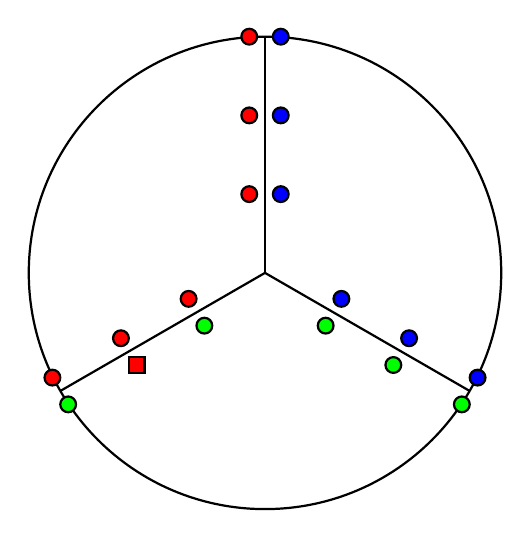
\begin{tikzpicture} [scale = 1] 
\draw[thick] (0.0, 0.0) circle [radius = 3.0];
\draw[thick] (0.0, 0.0) -- (0.0, 3.0);
\draw[fill = blue, thick] (0.2, 1.0) circle [radius = 0.1];
\draw[fill = blue, thick] (0.2, 2.0) circle [radius = 0.1];
\draw[fill = blue, thick] (0.2, 3.0) circle [radius = 0.1];
\draw[fill = red, thick] (-0.2, 1.0) circle [radius = 0.1];
\draw[fill = red, thick] (-0.2, 2.0) circle [radius = 0.1];
\draw[fill = red, thick] (-0.2, 3.0) circle [radius = 0.1];
\draw[thick] (0.0, 0.0) -- (2.6, -1.5);
\draw[fill = blue, thick] (0.97, -0.33) circle [radius = 0.1];
\draw[fill = blue, thick] (1.83, -0.83) circle [radius = 0.1];
\draw[fill = blue, thick] (2.7, -1.33) circle [radius = 0.1];
\draw[fill = green, thick] (0.77, -0.67) circle [radius = 0.1];
\draw[fill = green, thick] (1.63, -1.17) circle [radius = 0.1];
\draw[fill = green, thick] (2.5, -1.67) circle [radius = 0.1];
\draw[thick] (0.0, 0.0) -- (-2.6, -1.5);
\draw[fill = red, thick] (-0.97, -0.33) circle [radius = 0.1];
\draw[fill = red, thick] (-1.83, -0.83) circle [radius = 0.1];
\draw[fill = red, thick] (-2.7, -1.33) circle [radius = 0.1];
\draw[fill = green, thick] (-0.77, -0.67) circle [radius = 0.1];
\draw[fill = red, thick] (-1.73, -1.27) rectangle (-1.53, -1.07);
\draw[fill = green, thick] (-2.5, -1.67) circle [radius = 0.1];
\end{tikzpicture} \captionof{figure}{Incentive Incompatible Example}\label{fig:ice}
\end{figure}
The $18$ points are located inside a unit circle, and each point is $0.004$ away from the three line segments through the origin that forms angles of $120$ degrees between them. There is one red point, drawn as a square in the diagram, that is on the "incorrect" side of the boundary. For the agent represented by the red square, truthfully reporting her label will lead to a multi-class logistic regression model that classifies her point as "green". The probability that this model classifies her point as "red" is $0.3290$. However, if the agent misreports her label as "blue", the resulting model classifies her point as "red", and with a probability of $0.4966$. By lying about her label, the agent can make the principal learn an incorrect model that classifies her point correctly and with a higher probability.
\newline \newline
The example provides insight on the general incentive incompatibility issue of many classification models used in machine learning. The "red" agent that gets incorrectly classified as "green", does not want to misreport her label as "green", but instead has incentive to misreport her label as the third alternative "blue" to influence the classifier in a way that changes the decision between "red" and "green". Intuitively, if there are only two classes, then the agent would not be willing to misreport her label if the classifier is monotonic, in the sense that adding a point from one class increases the probability that this point is classified as a member of that class; and if there are more than two classes, then the agent would not be willing to misreport her label if the classifier is independent of irrelevant alternatives, in the sense that adding a point from a third class would not affect the decisions between the two classes.
\newline \newline
Previous work on mechanism design for machine learning with strategic data sources focus on designing robust algorithms to incentivize the data providers to report their private data truthfully. Their models mainly differ in the objective and the possible actions of the data providers (agents) and the learner (principal).
\newline \newline
The first group of papers focuses on principal-agent problems in which each agent's private data point is the agent's type that the agent cannot change. The only action the agents can take is whether to report their private information truthfully.
\begin{enumerate}
\item Some models assume the agents' feature vectors are public, but their labels are private. \citet*{perote2004strategy}, \citet*{chen2018strategyproof}, and \citet*{gast2013linear} focus on strategy-proof linear regression algorithms and introduced clockwise repeated median estimators, generalized resistant hyperplane estimators, and modified generalized linear squares estimators. \citet*{dekel2010incentive} investigates the general regression problem with empirical risk minimization and absolute value loss. All the previously mentioned papers assume the labels are continuous variables (regression problems), and \citet*{meir2012algorithms} assumes the labels are discrete variables (classification problems) and proposes a class of random dictator mechanisms.
\item Some models assume the agents' feature vectors are also private. \citet*{chen2019grinding} investigates such problems for linear regressions.
\item Other models do not distinguish between feature vectors and labels. Each agent has a private valuation. These problems are usually modeled as facility locations problems and the solution involves some variant of the Vickrey-Clarke-Groves or Meyerson auction. These include \citet*{dutting2017optimal}, \citet*{golowich2018deep}, \citet*{epasto2018incentive}, and \citet*{procaccia2009approximate}.
\end{enumerate}


The second group papers focus on moral-hazard problems in which each agent does not have a type but they can choose an action (with a cost) that affects the probability of obtaining the correct label. \citet*{richardsonprivately} focuses on the linear regression problem in this scenario, and \citet*{cai2015optimum} and \citet*{shah2016double} investigates the problem for more general machine learning problems. \citet*{mihailescu2010strategy} also discusses a similar problem for general machine learning algorithms.
\newline \newline
The last group of papers uses machine learning or robust statistics techniques without game-theoretic models. This group of papers include \citet*{dekel2009vox}, \citet*{dekel2009good}.
\newline \newline



\section{Logistic Regression} 

\subsection{Model}
In this section, we introduce the model using logistic regression as an example. We assume the principal is training a multi-class logistic (softmax) regression. There are $n $ strategic agents each providing the label of one data point to the principal. An agent, $i $, with public $x_{i} \in \mathbb{R}^{m}$, and private discrete $y_{i} \in \left\{1, 2, ..., k \right\}$, has the objective of maximizing the probability that her data point is labeled correctly by the principal's model, parameterized by the $m  \times \left(k  + 1\right)$ weights (and bias) matrix $w $. The agent can choose to report $y^{\dagger}_{i}$ to achieve the objective, with possibly $y^{\dagger}_{i} \neq  y_{i}$. Denoting the weights of the model resulting from the false report from agent $i $ by $w^\star \left(y^{\dagger}_{i}\right)$, and $w^{\dagger}$ when the agent the her report is clear, the agent's objective can be written as,
\begin{align*}
&  \displaystyle\max_{y^{\dagger} \in \left\{1, 2, ..., k \right\}} \mathbb{P}\left\{Y = y_{i} | w^\star \left(y^{\dagger}_{i}\right), x_{i}\right\},
\end{align*}
where,
\begin{align*}
&  \mathbb{P}\left\{Y = c | w, x_{i}\right\} = \dfrac{e^{z_{i,c}}}{\displaystyle\sum_{c'=1}^{k} e^{z_{i,c'}}},
\\ &  z_{i,c} = \displaystyle\sum_{j=1}^{m} w_{j,c} x_{i,j} + b_{c} , \text{\;for\;} c \in \left\{1, 2, ..., k\right\}.
\end{align*}
The principal is not strategic and he maximizes the likelihood of the data,
\begin{align*}
&\displaystyle\max_{w} \displaystyle\sum_{i=1}^{n} \log\left(\mathbb{P}\left\{Y = y^{\dagger}_{i} | w, x_{i}\right\}\right).
\end{align*}
We consider the case without a coalition of a group of agents, so only one agent is misreporting at a time, and use the following notations,
\begin{align*}
w^\star  &= \arg\displaystyle\max_{w} \displaystyle\sum_{i=1}^{n} \log\left(\mathbb{P}\left\{Y = y_{i} | x_{i}; w\right\}\right), \text{\;and\;}
\\ w^{\dagger} &= w^\star \left(y^{\dagger}_{i}\right) = \arg\displaystyle\max_{w} \log\left(\mathbb{P}\left\{Y = y^{\dagger}_{i} | x_{i}; w\right) + \displaystyle\sum_{i' = 0, i' \neq  i}^{n} \log\left(\mathbb{P}\left\{Y = y_{i'} | x_{i'}; w\right\}\right).\right.
\end{align*}
\begin{df} \label{df:ic} 
A dataset is incentive incompatible with respect to a classifier if there exists at least one agent $i $, and some $y^{\dagger}_{i} \neq  y_{i}$ such that,
\begin{align*}
\mathbb{P}\left\{Y = y_{i} | x_{i}; w^\star \right\} &< \mathbb{P}\left\{Y = y_{i} | x_{i}; w^\star \left(y^{\dagger}_{i}\right)\right\}.
\end{align*}
A classifier is incentive compatible if there does not exist a dataset that is incentive incompatible with respect to the classifier.
\newline \newline\end{df}
\begin{conj} \label{conj:logit} 
Multi-class logistic regression is not incentive compatible.
\newline \newline\end{conj}
The example described in Figure \ref{fig:ice} is a dataset that is numerically incentive incompatible.
\\* In this example, agent $i $ reports $x_{i} \in \mathbb{R}^{2}$ and $y_{i}$ is one of $1$ (red), $2$ (green), or $3$ (blue). Suppose the red square point correspond to agent $1$ with $x_{1} = \left(-1.63, -1.17\right)$ and $y_{1} = 1$.
\begin{align*}
\mathbb{P}\left\{Y = 1 | w^\star , x_{1}\right\} &= 0.3290,
\\ \mathbb{P}\left\{Y = 1 | w^\star \left(y^{\dagger}_{1} = 3\right), x_{1}\right\} &= 0.4966.
\end{align*}
Here, parameter estimation is done using maximum likelihood estimation with BFGS, and $w^\star $ is given by, with class $1$ weights normalized to $0$,

\begin{center} \begin{tabular}{|c|c|c|c|c|}
\hline
 Class &(Intercept) &x1 &x2\\ \hline
$2$ &-$0.6053178$ &$104.9925$ &-$181.3391914$\\ \hline
$3$ &-$0.2852057$ &$209.4190$ &$0.3656777$\\ \hline
\end{tabular} \end{center}
and $w^\star \left(y^{\dagger}_{1} = 3\right)$ is given by,

\begin{center} \begin{tabular}{|c|c|c|c|c|}
\hline
 Class &(Intercept) &x1 &x2\\ \hline
$2$ &-$0.1915645$ &$3.473426$ &-$5.507418$\\ \hline
$3$ &$0.8273350$ &$4.309293$ &-$1.200060$\\ \hline
\end{tabular} \end{center}
Using BFGS to maximize likelihood leads to the same incentive incompatibility result. Currently there is no formal proof that the result is not due to numerical instability, therefore, @(logit) is stated as a conjecture. Numerical experiments indicates that incentive incompatible datasets are rare. If the data points are two dimensional and standard normally distributed, and the labels are created using randomly generated weights with a small probability of error, then such a dataset is incentive incompatible with a probability of $0.005$.
\newline \newline


\subsection{Binary Classification}
\begin{prop} \label{prop:bin} 
Binary empirical risk minimization (ERM) classifiers are incentive compatible.
\end{prop}
\begin{proof} \label{proof:binpf} 
For any dataset $\left\{\left(x_{i}, y_{i}\right)\right\}_{i=1}^{n}$, and the hypothesis class $\mathcal{H}$, let the optimal classifier in the case every agent report truthfully be,
\begin{align*}
h^\star  &= \arg\displaystyle\min_{h \in \mathcal{H}} \displaystyle\sum_{i'=1}^{n} \ell\left(h, x_{i'}, y_{i'}\right).
\end{align*}
Fix an agent $i $, her feature vector $x_{i}$, and fix other agents' reports, $\left(x_{-i}, y_{-i}\right)$, define the optimal classifier given the classifier $h $ and the misreport of agent $i , y^{\dagger}_{i} = 1 - y_{i}$ as,
\begin{align*}
h^\star \left(y^{\dagger}_{i}\right) &= \arg\displaystyle\min_{h \in \mathcal{H}} \displaystyle\sum_{i'=1, i' \neq  i}^{n} \ell\left(h, x_{i'}, y_{i'}\right) + \ell\left(h, x_{i}, y^{\dagger}_{i}\right).
\end{align*}
Now suppose, for a contradiction, that agent $i $ prefers misreporting,
\begin{align*}
\ell\left(h^\star , x_{i}, y_{i}\right) &> \ell\left(h^\star \left(y^{\dagger}_{i}\right), x_{i}, y_{i}\right),
\end{align*}
which implies, since $y^{\dagger}_{i} = 1 - y_{i,}$
\begin{align*}
\ell\left(h^\star , x_{i}, y^{\dagger}_{i}\right) &< \ell\left(h^\star \left(y^{\dagger}_{i}\right), x_{i}, y^{\dagger}_{i}\right).
\end{align*}
Note that the above implication only works for binary classification.
\\* Due to the optimality of $h^\star \left(y^{\dagger}_{i}\right)$,
\begin{align*}
\displaystyle\sum_{i'=1, i' \neq  i}^{n} \ell\left(h^\star \left(y^{\dagger}_{i}\right), x_{i'}, y_{i'}\right) + \ell\left(h^\star \left(y^{\dagger}_{i}\right), x_{i}, y^{\dagger}_{i}\right) &\leq  \displaystyle\sum_{i'=1, i' \neq  i}^{n} \ell\left(h^\star , x_{i'}, y_{i'}\right) + \ell\left(h^\star , x_{i}, y^{\dagger}_{i}\right),
\end{align*}
using the above inequalities, the comparison can be simplified to,
\begin{align*}
\displaystyle\sum_{i'=1, i' \neq  i}^{n} \ell\left(h^\star \left(y^{\dagger}_{i}\right), x_{i'}, y_{i'}\right) &\leq  \displaystyle\sum_{i'=1, i' \neq  i}^{n} \ell\left(h^\star , x_{i'}, y_{i'}\right),
\\ \displaystyle\sum_{i'=1}^{n} \ell\left(h^\star \left(y^{\dagger}_{i}\right), x_{i'}, y_{i'}\right) &\leq  \displaystyle\sum_{i'=1}^{n} \ell\left(h^\star , x_{i'}, y_{i'}\right),
\end{align*}
which is a contradiction to the optimality of $h^\star $.
\newline \newline\end{proof}


\subsection{Zero-One Loss Logistic Regression}
It is, however, possible to change the loss function so that logistic regression is incentive compatible. Changing the loss function to absolute value $L^{1}$ loss is one possibility, due to \citet*{dekel2010incentive}. Their result on incentive compatibility of empirical risk minimization in the regression setting is applicable in our model. In addition to absolute value loss, which is not a meaningful loss function for multi-class logistic regression, zero-one loss logistic regression with deterministic predictions is also incentive compatible.
\newline \newline
\begin{prop} \label{prop:zolog} 
Multi-class deterministic empirical risk minimization classifiers with zero-one loss are incentive compatible.
\end{prop}
\begin{proof} \label{proof:zologpf} 
For any dataset $\left\{\left(x_{i}, y_{i}\right)\right\}_{i=1}^{n}$, and the hypothesis class $\mathcal{H}$, let the optimal classifier be,
\begin{align*}
h^\star  &= \arg\displaystyle\min_{h \in \mathcal{H}} \displaystyle\sum_{i'=1}^{n} \mathbbm{1}_{\left\{y_{i'} \neq  h\left(x_{i'}\right)\right\}}.
\end{align*}
Fix an agent $i $, her feature vector $x_{i}$, and fix other agents' reports, $\left(x_{-i}, y_{-i}\right)$, define the loss function given the classifier $h $ and report of agent $i , y^{\dagger}_{i}$ as,
\begin{align*}
\mathcal{L}\left(h, y^{\dagger}_{i}\right) &= \displaystyle\sum_{i' \neq  i} \mathbbm{1}_{\left\{y_{i'} \neq  h\left(x_{i'}\right)\right\}} + \mathbbm{1}_{\left\{y^{\dagger}_{i} \neq  h\left(x_{i}\right)\right\}}.
\end{align*}
If $y_{i} = h^\star \left(x_{i}\right)$, then the classifier is already classifying $x_{i}$ correctly, misreporting will not improve the outcome for $i $. Now let the prediction be $h^\star \left(x_{i}\right) = y^\star  \neq  y_{i}$, and suppose $h^\star $ is making $k $ mistakes, meaning,
\begin{align*}
k  &= \displaystyle\min_{h \in \mathcal{H}} \mathcal{L}\left(h^\star , y_{i}\right).
\end{align*}
Agent $i $ can misreport in the following two ways:
\end{proof}
\begin{enumerate}
\item If agent $i $ reports $y^{\dagger}_{i} = y^\star $, let the new classifier be $h^{\dagger}$, note that we must have,
\begin{align*}
\mathcal{L}\left(h^{\dagger}, y^\star \right) &\leq  k - 1,
\end{align*}
because $\mathcal{L}\left(h^{\dagger}, y^\star \right) > k - 1 = \mathcal{L}\left(h^\star , y^\star \right)$ contradicts the optimality of $h^{\dagger.}$
\\* Now suppose that agent $i $ could get her true label with $h^{\dagger}$, meaning $h^{\dagger}\left(x_{i}\right) = y_{i}$, then,
\begin{align*}
\mathcal{L}\left(h^{\dagger}, y_{i}\right) &= \mathcal{L}\left(h^{\dagger}, y^\star \right) - 1
\\ &\leq  k - 2
\\ &< \mathcal{L}\left(h^\star , y_{i}\right),
\end{align*}
which contradicts the optimality of $h^\star $. Therefore, agent $i $ cannot improve the outcome by misreporting $y^\star $.
\item If agent $i $ reports $y^{\dagger}_{i} = y' \neq  y^\star $, let the new classifier be $h^{\dagger}$, note that we must have,
\begin{align*}
\mathcal{L}\left(h^{\dagger}, y'\right) &\leq  k,
\end{align*}
because if $\mathcal{L}\left(h^{\dagger}, y'\right) > k = \mathcal{L}\left(h^\star , y'\right)$ contradicts the optimality of $h^{\dagger.}$
\\* Now suppose that agent $i $ could get her true label with $h^{\dagger}$, then,
\begin{align*}
\mathcal{L}\left(h^{\dagger}, y_{i}\right) &= \mathcal{L}\left(h^{\dagger}, y_{i}\right) - 1
\\ &\leq  k - 1
\\ &< \mathcal{L}\left(h^\star , y_{i}\right),
\end{align*}
which contradicts the optimality of $h^\star $. Therefore, agent $i $ cannot improve the outcome by misreporting $y'$.
\\* Therefore, no agent can improve the outcome and the dataset is incentive compatible.
\newline \newline
\end{enumerate}




\section{Other Classifiers} 

\subsection{Bayes Classifiers}
The example given previously is incentive compatible with respect to the Naive Bayes classifier. None of the agents have the incentive to misreport their labels. This is always true in general for any parametric Bayes classifier estimated using maximum likelihood.
\newline \newline
\begin{lem} \label{lem:bc} 
Bayes classifiers estimated by maximum likelihood are incentive compatible.
\end{lem}
\begin{proof} \label{proof:bcpf} 
Suppose the loglikelihood function of class $y $ given the feature vector $x $ and the parameter $w $ is $\ell\left(x ; w \right)$, and define the optimal parameter, $w^\star $ for class $y_{i}$, of the truthful model as,
\begin{align*}
w^\star  &= \arg\displaystyle\max_{w} \displaystyle\sum_{i' : y_{i'} = y_{i}} \ell\left(x_{i'} ; w\right)
\\ &= \arg\displaystyle\max_{w} \displaystyle\sum_{i' \neq  i : y_{i'} = y_{i}} \ell\left(x_{i'} ; w\right) + \ell\left(x_{i} ; w\right).
\end{align*}
Let the optimal parameter when agent $i $ reports $y^{\dagger}_{i} \neq  y_{i}$ be $w^{\dagger,}$
\begin{align*}
w^{\dagger} &= \arg\displaystyle\max_{w} \displaystyle\sum_{i' \neq  i: y_{i'} = y_{i}} \ell\left(x_{i'} ; w\right).
\end{align*}
In particular, these implies the following optimality conditions,
\begin{align*}
\displaystyle\sum_{i' \neq  i : y_{i'} = y_{i}} \ell\left(x_{i'} ; w^\star \right) + \ell\left(x_{i} ; w^\star \right) &\geq  \displaystyle\sum_{i' \neq  i : y_{i'} = y_{i}} \ell\left(x_{i'} ; w^{\dagger}\right) + \ell\left(x_{i} ; w^{\dagger}\right),
\\ \displaystyle\sum_{i' \neq  i: y_{i'} = y_{i}} \ell\left(x_{i'} ; w^{\dagger}\right) &\geq  \displaystyle\sum_{i' \neq  i: y_{i'} = y_{i}} \ell\left(x_{i'}, w^\star \right).
\end{align*}
Taking the difference between the two inequalities, we have,
\begin{align*}
\ell\left(x_{i} ; w^\star \right) &\geq  \ell\left(x_{i} ; w^{\dagger}\right).
\end{align*}
Note that the empirical prior probability for class $y_{i}$ is decreased if the number of data with label $y_{i}$ is decreased by $1$. Therefore, the posterior probabilities satisfy,
\begin{align*}
\mathbb{P}\left\{y_{i} | x_{i}, w^\star \right\} &\geq  \mathbb{P}\left\{y_{i} | x_{i}, w^{\dagger}\right\}.
\end{align*}
Therefore, no agent can improve the outcome and the dataset is incentive compatible.
\newline \newline\end{proof}
One special case of this is the Bayes classifier for the Gaussian Mixture Model.
\newline \newline


\subsection{Kernel Density Estimators}
There are two general approaches to use kernel densities for classification, the first is to use all the points to estimate the density and the second is to estimate the densities for each class separately (see \citet*{taylor1997classification}).
\newline \newline
The first approach suggests that,
\begin{align*}
\mathbb{P}\left\{X = x\right\} &= \dfrac{1}{n h^{D}} \displaystyle\sum_{i'=1}^{n} w_{i'}, \text{\;where\;} w_{i'} = K\left(\dfrac{x - x_{i'}}{h}\right).
\end{align*}
Define $w^\star $ to be the weight function when all agents report truthfully, then the classification probabilities for agent $i $ from dividing up the sum based on the class is,
\begin{align*}
\mathbb{P}\left\{Y = y_{i}, X = x_{i} | w^\star \right\} &= \dfrac{1}{n} \displaystyle\sum_{i'=1}^{n} w^\star _{i'} \mathbbm{1}_{\hat{y}_{i'} = y_{i}}
\\ &= \dfrac{1}{n} \displaystyle\sum_{i'=1}^{n} w^\star _{i'} \mathbbm{1}_{\hat{y}_{i'} = y_{i}, i' \neq  i} + \dfrac{1}{n} w^\star _{i}
\\ &= \mathbb{P}\left\{Y = y_{i}, X = x_{i} | w^\star \left(y^{\dagger}_{i}\right)\right\} + \dfrac{1}{n} K\left(0\right), \text{\;since\;} y^{\dagger}_{i} \neq  y_{i}
\\ &\leq  \mathbb{P}\left\{Y = y_{i}, X = x_{i} | w^\star \left(y^{\dagger}_{i}\right)\right\},
\end{align*}
meaning reporting truthfully results in a larger probability compared to reporting $y^{\dagger}_{i}$ instead.
\newline \newline
Alternative if the classification probabilities are computed based on \citet*{taylor1997classification},
\begin{align*}
\mathbb{P}\left\{X = x | Y = y\right\} &= \dfrac{1}{n_{y} h^{D}} \displaystyle\sum_{i'=1}^{n} w_{i'} \mathbbm{1}_{\hat{y}_{i'} = y}, n_{y} = \displaystyle\sum_{i'=1}^{n} \mathbbm{1}_{\hat{y}_{i'} = y}
\end{align*}
Similar to the above derivation (and also as a special case of a Bayes estimator),
\begin{align*}
\mathbb{P}\left\{Y = y_{i}, X = x_{i} | w^\star \right\} &= \dfrac{1}{n_{y}} \displaystyle\sum_{i'=1}^{n} w^\star _{i'} \mathbbm{1}_{\hat{y}_{i'} = y_{i}}
\\ &= \mathbb{P}\left\{Y = y_{i}, X = x_{i} | w^\star \left(y^{\dagger}_{i}\right)\right\} + \dfrac{1}{n_{y}} K\left(0\right)
\\ &\leq  \mathbb{P}\left\{Y = y_{i}, X = x_{i} | w^\star \left(y^{\dagger}_{i}\right)\right\}.
\end{align*}
The above results will be referenced as the following lemma.
\newline \newline
\begin{lem} \label{lem:kde} 
Kernel density estimators are incentive compatible.
\newline \newline\end{lem}
K-Nearest Neighbor is a special case of this with a uniform kernel.
\newline \newline


\subsection{Artificial Examples}
One intuition behind why the above classifiers are always incentive-compatible is that one-vs-one classification decisions are made independently for classifiers. The classifiers like logistic regression have highly interdependent one-vs-one decisions. The following example is one in which $1$-vs-$2$ decisions are completely determined by the $2$-vs-$3$ decisions, and as a result, a class-$1$ point that is misclassified as class-$2$ could misreport as class-$3$ to influence the $2$-vs-$3$ decision boundary and indirectly change the $1$-vs-$2$ decision boundary in its favor.
\newline \newline
Consider the three-class $1D$ threshold classifiers in the form,
\[ \hat{y}\left(x; t\right) =\left\{ \begin{array}{ll}
1& \text{\;if\;} x < -t \\
2& \text{\;if\;} -t \leq  x \leq  t \\
3& \text{\;if\;} x > t \\
\end{array}\right. \]
This is effectively a one-vs-one threshold classifier with the $1$-vs-$2$ threshold of $-t $, with the $2$-vs-$3$ threshold of $t $ and the $1$-vs-$3$ threshold of any value between $-t $ and $t $. Now define the loss function as the squared error margin,
\[ \ell\left(x_{i}, y_{i}; t\right) =\left\{ \begin{array}{ll}
\left(x_{i} - \left(-t\right)\right)^{2} \mathbbm{1}_{\hat{y}\left(x_{i}; t\right) \neq  y_{i}}& \text{\;if\;} y_{i} = 1 \\
\displaystyle\min\left\{\left(x_{i} - \left(-t\right)\right)^{2}, \left(x_{i} - t\right)^{2}\right\} \mathbbm{1}_{\hat{y}\left(x_{i}; t\right) \neq  y_{i}}& \text{\;if\;} y_{i} = 2 \\
\left(x_{i} - t\right)^{2} \mathbbm{1}_{\hat{y}\left(x_{i}; t\right) \neq  y_{i}}& \text{\;if\;} y_{i} = 3 \\
\end{array}\right. \]
Then, the learner's maximization problem is,
\begin{align*}
&\displaystyle\min_{t \in \mathbb{R}} \ell\left(x_{i}, y_{i}; t\right).
\end{align*}
The agents' problem is to minimize the loss for their point with their true label. The loss can be either the margin loss or zero-one loss, here, for simplicity, assume the agents also want to minimize the margin,
\begin{align*}
&\displaystyle\max_{y^{\dagger}_{i} \in \left\{1, 2, 3\right\}} \ell\left(x_{i}, y_{i}; t^\star \left(y^{\dagger}_{i}\right)\right),
\end{align*}
where $t^\star \left(y^{\dagger}_{i}\right)$ is the optimal threshold $t $ for the learner when agent $i $ misreports the label as $y^{\dagger}_{i.}$
\\* For the dataset $\left\{\left(x_{i}, y_{i}\right)\right\}_{i=1}^{5} = \left\{\left(-4, 1\right), \left(-3, 2\right), \left(-2, 1\right), \left(3, 2\right), \left(4, 3\right)\right\}$, the minimum loss is $1$ and it occurs when $t  = 3$ when every agent reports truthfully. In this case, agent (-$2, 1$) is misclassified as (-$2, 2$). However, if (-$2, 1$) misreports as (-$2, 3$), the loss from $t  = 3$ is $25$ and the minimum loss is $22$ and it occurs when $t  = 0$. In this case, agent (-$2, 1$) is classified correctly. In particular, the agent (-$2, 1$) improves the loss from $1$ to $0$.
\newline \newline

\begin{figure}[H] \centering 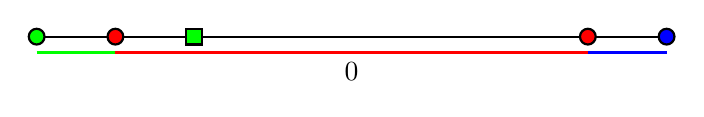
\begin{tikzpicture} [scale = 1] 
\draw[thick] (-4.0, 0.0) -- (4.0, 0.0);
\draw[fill = green, thick] (-4.0, 0.0) circle [radius = 0.1];
\draw[fill = green, thick] (-2.1, -0.1) rectangle (-1.9, 0.1);
\draw[fill = red, thick] (-3.0, 0.0) circle [radius = 0.1];
\draw[fill = red, thick] (3.0, 0.0) circle [radius = 0.1];
\draw[fill = blue, thick] (4.0, 0.0) circle [radius = 0.1];
\draw[green, thick] (-4.0, -0.2) -- (-3.0, -0.2);
\draw[red, thick] (-3.0, -0.2) -- (3.0, -0.2);
\draw[blue, thick] (3.0, -0.2) -- (4.0, -0.2);
\node[below] at (0.0, -0.2){$0$};
\end{tikzpicture} \captionof{figure}{$1D$ Artificial Incentive Incompatible Example (Truthful)}\label{fig:1dat}
\end{figure}

\begin{figure}[H] \centering 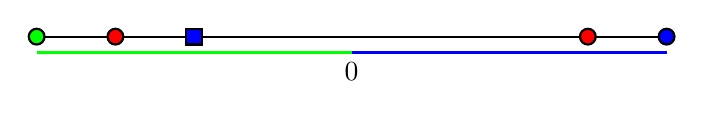
\begin{tikzpicture} [scale = 1] 
\draw[thick] (-4.0, 0.0) -- (4.0, 0.0);
\draw[fill = green, thick] (-4.0, 0.0) circle [radius = 0.1];
\draw[fill = blue, thick] (-2.1, -0.1) rectangle (-1.9, 0.1);
\draw[fill = red, thick] (-3.0, 0.0) circle [radius = 0.1];
\draw[fill = red, thick] (3.0, 0.0) circle [radius = 0.1];
\draw[fill = blue, thick] (4.0, 0.0) circle [radius = 0.1];
\draw[green, thick] (-4.0, -0.2) -- (0.0, -0.2);
\draw[red, thick] (0.0, -0.2) -- (0.0, -0.2);
\draw[blue, thick] (0.0, -0.2) -- (4.0, -0.2);
\node[below] at (0.0, -0.2){$0$};
\end{tikzpicture} \captionof{figure}{$1D$ Artificial Incentive Incompatible Example (Misreport)}\label{fig:1dam}
\end{figure}
Intuitively, when the misclassified class-$1$ point pretends to be a class-$3$ point with a large loss, the classifier modifies the $2$-vs-$3$ decision boundary to minimize that loss and the point benefits from the interdependence between the $2$-vs-$3$ decision and the $1$-vs-$2$ decision.
\newline \newline
To generalize the above observations, suppose the learner is a probabilistic classifier with parameters estimated by maximum likelihood, and the agents report their labels to maximize the classification probability of their true labels. Then the following two conditions guarantee that the classification is incentive compatible.
\newline \newline
\begin{df} \label{df:mono} 
(Monotonic Condition) A multi-class probabilistic classifier is monotonic if, given a training set $S $, for any point $x $ with labels $a $ and $b, $
\begin{align*}
\dfrac{\mathbb{P}\left\{Y = a | x, w^\star \left(S\right)\right\}}{\mathbb{P}\left\{Y = b | x, w^\star \left(S\right)\right\}} &\geq  \dfrac{\mathbb{P}\left\{Y = a | x, w^\star \left(S \cup \left\{\left(x, y = a\right)\right\}\right)\right\}}{\mathbb{P}\left\{Y = b | x, w^\star \left(S \cup \left\{\left(x, y = a\right)\right\}\right)\right\}}.
\end{align*}\end{df}
The assumption says that the probability that $x $ is classified as $a $ increases when there is an additional point $\left(x , a \right)$ in the training set.
\newline \newline
\begin{df} \label{df:iia} 
(Independence of Irrelevant Alternatives (IIA) Condition) A multi-class classifier is independent of irrelevant alternatives if, given a training set $S $, for any point $x $ and any pair of labels $a $ and $b, $
\begin{align*}
\dfrac{\mathbb{P}\left\{Y = a | x, w^\star \left(S\right)\right\}}{\mathbb{P}\left\{Y = b | x, w^\star \left(S\right)\right\}} &= \dfrac{\mathbb{P}\left\{Y = a | x, w^\star \left(S \cup \left\{\left(x', y' \notin \left\{a, b\right\}\right)\right\}\right)\right\}}{\mathbb{P}\left\{Y = b | x, w^\star \left(S \cup \left\{\left(x', y' \notin \left\{a, b\right\}\right)\right\}\right)\right\}}.
\end{align*}\end{df}
The assumption says that the ratio between the classification probabilities of $x $ of any two classes is not changed by adding a point at $x $ with a third class.
\newline \newline
Combining the two assumptions MC and IIA, we have that an agent with label $a $ cannot change the decision of $a $ vs $b $ by misreporting its label as a third class $c $. This observation is formalized in the following proposition.
\newline \newline
\begin{thm} \label{thm:margin} 
Multi-class probabilistic classifiers estimated by maximum likelihood is incentive compatible if it is monotonic and independent of irrelevant alternatives.
\end{thm}
\begin{proof} \label{proof:marginpf} 
Fix a dataset $\left\{\left(x_{i}, y_{i}\right)\right\}_{i=1}^{n}$, let the maximum likelihood estimates in the case every agent report truthfully be,
\begin{align*}
w^\star  &= \arg\displaystyle\max_{w} \displaystyle\sum_{i'=1}^{n} \log\left(\mathbb{P}\left\{Y = y_{i'} | x_{i'}, w\right\}\right).
\end{align*}
Fix an agent $i $, her feature vector $x_{i}$, and fix other agents' reports, $\left(x_{-i}, y_{-i}\right)$, define the maximum likelihood estimate given the misreport of agent $i , y^{\dagger}_{i}$ as,
\begin{align*}
w^{\dagger} &= \arg\displaystyle\max_{w} \displaystyle\sum_{i'=1, i' \neq  i}^{n} \log\left(\mathbb{P}\left\{Y = y_{i'} | x_{i'}, w\right\}\right) + \log\left(\mathbb{P}\left\{Y = y^{\dagger}_{i} | x_{i}, w\right\}\right).
\end{align*}
Now suppose, for a contradiction, that agent $i $ prefers misreporting, assume the following incentive inequality,
\begin{align*}
\mathbb{P}\left\{Y = y_{i} | x_{i}, w^\star \right\} &> \mathbb{P}\left\{Y = y_{i} | x_{i}, w^{\dagger}\right\}.
\end{align*}
If there are only two classes, then by symmetry,
\begin{align*}
\mathbb{P}\left\{Y = y^{\dagger}_{i} | x_{i}, w^\star \right\} &< \mathbb{P}\left\{Y = y^{\dagger}_{i} | x_{i}, w^{\dagger}\right\}.
\end{align*}
If there are more than two classes, fix a third $y'_{i} \notin \left\{y_{i}, y^{\dagger}_{i}\right\}$, and define an intermediate maximum likelihood estimate from removing the point $\left(x_{i}, y_{i}\right)$,
\begin{align*}
w' &= \arg\displaystyle\max_{w} \displaystyle\sum_{i'=1, i' \neq  i}^{n} \log\left(\mathbb{P}\left\{Y = y_{i'} | x_{i'}, w\right\}\right),
\end{align*}
then the Monotonic Condition implies,
\begin{align*}
\dfrac{\mathbb{P}\left\{Y = y_{i} | x_{i}, w^\star \right\}}{\mathbb{P}\left\{Y = y'_{i} | x_{i}, w^\star \right\}} &\leq  \dfrac{\mathbb{P}\left\{Y = y_{i} | x_{i}, w'\right\}}{\mathbb{P}\left\{Y = y'_{i} | x_{i}, w'\right\}},
\end{align*}
and the IIA Condition implies,
\begin{align*}
\dfrac{\mathbb{P}\left\{Y = y_{i} | x_{i}, w'\right\}}{\mathbb{P}\left\{Y = y'_{i} | x_{i}, w'\right\}} &= \dfrac{\mathbb{P}\left\{Y = y_{i} | x_{i}, w^{\dagger}\right\}}{\mathbb{P}\left\{Y = y'_{i} | x_{i}, w^{\dagger}\right\}}.
\end{align*}
Combining the above two inequalities with the incentive inequality, we have,
\begin{align*}
\mathbb{P}\left\{Y = y'_{i} | x_{i}, w^\star \right\} &> \mathbb{P}\left\{Y = y'_{i} | x_{i}, w^{\dagger}\right\}.
\end{align*}
Note that the above inequality is true for all $y'_{i} \notin \left\{y_{i}, y^{\dagger}_{i}\right\}$, summing over all such $y'_{i}$ results in,
\begin{align*}
\displaystyle\sum_{y \notin \left\{y_{i}, y^{\dagger}_{i}\right\}} \mathbb{P}\left\{Y = y'_{i} | x_{i}, w^\star \right\} &> \displaystyle\sum_{y \notin \left\{y_{i}, y^{\dagger}_{i}\right\}} \mathbb{P}\left\{Y = y'_{i} | x_{i}, w^{\dagger}\right\},
\end{align*}
given that the class probabilities sum up to $1$,
\begin{align*}
1 - \mathbb{P}\left\{Y = y_{i} | x_{i}, w^\star \right\} - \mathbb{P}\left\{Y = y^{\dagger}_{i} | x_{i}, w^\star \right\} &> 1 - \mathbb{P}\left\{Y = y_{i} | x_{i}, w^{\dagger}\right\} - \mathbb{P}\left\{Y = y^{\dagger}_{i} | x_{i}, w^{\dagger}\right\},
\end{align*}
and using the incentive inequality again,
\begin{align*}
\mathbb{P}\left\{Y = y^{\dagger}_{i} | x_{i}, w^\star \right\} &< \mathbb{P}\left\{Y = y^{\dagger}_{i} | x_{i}, w^{\dagger}\right\}.
\end{align*}
Now, due to the optimality of $h^{\dagger,}$
\begin{align*}
&  \displaystyle\sum_{i'=1, i' \neq  i}^{n} \log\left(\mathbb{P}\left\{Y = y_{i'} | x_{i'}, w^{\dagger}\right\}\right) + \log\left(\mathbb{P}\left\{Y = y^{\dagger}_{i} | x_{i}, w^{\dagger}\right\}\right)
\\ &\leq  \displaystyle\sum_{i'=1, i' \neq  i}^{n} \log\left(\mathbb{P}\left\{Y = y_{i'} | x_{i'}, w^\star \right\}\right) + \log\left(\mathbb{P}\left\{Y = y^{\dagger}_{i} | x_{i}, w^\star \right\}\right),
\end{align*}
using the above inequalities, the comparison can be simplified to,
\begin{align*}
\displaystyle\sum_{i'=1, i' \neq  i}^{n} \log\left(\mathbb{P}\left\{Y = y_{i'} | x_{i'}, w^{\dagger}\right\}\right) &< \displaystyle\sum_{i'=1, i' \neq  i}^{n} \log\left(\mathbb{P}\left\{Y = y_{i'} | x_{i'}, w^\star \right\}\right),
\\ \displaystyle\sum_{i'=1}^{n} \log\left(\mathbb{P}\left\{Y = y_{i'} | x_{i'}, w^{\dagger}\right\}\right) &< \displaystyle\sum_{i'=1}^{n} \log\left(\mathbb{P}\left\{Y = y_{i'} | x_{i'}, w^\star \right\}\right),
\end{align*}
which is a contradiction to the optimality of $w^\star $.
\newline \newline\end{proof}
The assumptions Definition \ref{df:mono} (MC) and Definition \ref{df:iia} (IIA) can be significantly simplified for a separable class of the classifiers.
\newline \newline
\begin{df} \label{df:sep} 
A probabilistic classifier is separable if the parameters $w^\star $ can be partitioned into $K $ classes, $w^\star _{1}, w^\star _{2}, ..., w^\star _{K}$, one set of parameters for each class, such that for given training sets $S $ and $S'$ and any label $k $ if,
\begin{align*}
\left\{\left(x_{i}, y_{i}\right) \in S : y_{i} = k\right\} &= \left\{\left(x_{i}, y_{i}\right) \in S' : y_{i} = k\right\},
\end{align*}
then,
\begin{align*}
w^\star _{k}\left(S\right) &= w^\star _{k}\left(S'\right),
\end{align*}
and if there is a value function $v_{k}\left(x\right)$ that only depends on $w^\star _{k}$ such that,
\begin{align*}
\mathbb{P}\left\{Y = y | x; w^\star \right\} &= \dfrac{v_{k}\left(x\right)}{\displaystyle\sum_{k' = 1}^{K} v_{k'}\left(x\right)},
\end{align*}
then the classifier is separable.
\newline \newline\end{df}
For separable classifiers, Definition \ref{df:iia} (IIA) is always satisfied since we have, for any label $a, $
\begin{align*}
\mathbb{P}\left\{Y = a|x, w^\star \left(S\right)\right\} &= \mathbb{P}\left\{Y = a|x, w^\star _{a}\left(S\right)\right\} = \mathbb{P}\left\{Y = a|x, w^\star _{a}\left(S \cup \left\{\left(x, y \neq  a\right)\right\}\right)\right\},
\end{align*}
and Definition \ref{df:mono} (MC) is reduced to the following inequality,
\begin{align*}
\mathbb{P}\left\{Y = a | x, w^\star \left(S\right)\right\} &\geq  \mathbb{P}\left\{Y = a | x, w^\star \left(S \cup \left\{\left(x, y = a\right)\right\}\right)\right\},
\end{align*}
which is always true implied by the difference between the optimality conditions of $w^\star \left(S\right)$ and $w^\star \left(S \cup \left\{\left(x, y = a\right)\right\}\right)$.
\newline \newline
\begin{cor} \label{cor:sepmargin} 
A separable multi-class probabilistic classifier estimated by maximum likelihood is incentive compatible.
\newline \newline\end{cor}
It immediately follows Lemma \ref{lem:bc} and Lemma \ref{lem:kde} hold, because the parameters for different classes are estimated separately, and the probabilities are computed as proportions.
\newline \newline
A similar result can be obtained for empirical risk minimization. We could either add an assumption that the loss function can be normalized so that the sum is constant and it behaves the same way as a probabilistic classifier, or we could use stronger Monotonic and IIA Conditions.
\newline \newline
\begin{df} \label{df:nrml} 
(Normalized Loss) A loss function $\ell$ is normalized if given a hypothesis $h $, for any point $x, $
\begin{align*}
\displaystyle\sum_{y} \ell\left(h, x, y\right) &= C , \text{\;constant\;} .
\end{align*}\end{df}
\begin{df} \label{df:monoerm} 
(Monotonic Condition for ERM) Multi-class empirical risk minimization classifiers are monotonic if, given a training set $S $, for any point $x $ with labels $a $ and $b, $
\begin{align*}
\dfrac{\ell\left(h^\star \left(S\right), x, y = a\right)}{\ell\left(h^\star \left(S\right), x, y = b\right)} &\geq  \dfrac{\ell\left(h^\star \left(S \cup \left\{\left(x, y = a\right)\right\}\right), x, y = a\right)}{\ell\left(h^\star \left(S \cup \left\{\left(x, y = a\right)\right\}\right), x, y = b\right)}.
\end{align*}\end{df}
\begin{df} \label{df:iiaerm} 
(IIA Condition for ERM) Multi-class empirical risk minimization classifiers are independent of irrelevant alternatives if, given a training set $S $, for any point $x $ and any pair of labels $a $ and $b, $
\begin{align*}
\dfrac{\ell\left(h^\star \left(S\right), x, y = a\right)}{\ell\left(h^\star \left(S\right), x, y = b\right)} &= \dfrac{\ell\left(h^\star \left(S \cup \left\{\left(x', y' \notin \left\{a, b\right\}\right)\right\}\right), x, y = a\right)}{\ell\left(h^\star \left(S \cup \left\{\left(x', y' \notin \left\{a, b\right\}\right)\right\}\right), x, y = b\right)}.
\end{align*}\end{df}
\begin{cor} \label{cor:marginerm} 
Multi-class empirical risk minimization classifiers with normalized loss functions are incentive compatible if it is monotonic and independent of irrelevant alternatives.
\end{cor}
\begin{proof} \label{proof:marginermpf} 
For a fixed dataset $\left\{\left(x_{i}, y_{i}\right)\right\}_{i=1}^{n}$, and the hypothesis class $\mathcal{H}$, let the optimal classifier in the case every agent report truthfully be,
\begin{align*}
h^\star  &= \arg\displaystyle\min_{h \in \mathcal{H}} \displaystyle\sum_{i'=1}^{n} \ell\left(h, x_{i'}, y_{i'}\right).
\end{align*}
Fix an agent $i $, her feature vector $x_{i}$, and fix other agents' reports, $\left(x_{-i}, y_{-i}\right)$, define the optimal classifier given the classifier $h $ and the misreport of agent $i , y^{\dagger}_{i}$ as,
\begin{align*}
h^{\dagger} &= \arg\displaystyle\min_{h \in \mathcal{H}} \displaystyle\sum_{i'=1, i' \neq  i}^{n} \ell\left(h, x_{i'}, y_{i'}\right) + \ell\left(h, x_{i}, y^{\dagger}_{i}\right).
\end{align*}
Now suppose, for a contradiction, that agent $i $ prefers misreporting, assume the following incentive inequality,
\begin{align*}
\ell\left(h^\star , x_{i}, y_{i}\right) &> \ell\left(h^{\dagger}, x_{i}, y_{i}\right).
\end{align*}
If there are only two classes, then by symmetry,
\begin{align*}
\ell\left(h^\star , x_{i}, y^{\dagger}_{i}\right) &< \ell\left(h^{\dagger}, x_{i}, y^{\dagger}_{i}\right).
\end{align*}
If there are more than two classes, fix a third $y'_{i} \notin \left\{y_{i}, y^{\dagger}_{i}\right\}$, and define an intermediate maximum likelihood estimate from removing the point $\left(x_{i}, y_{i}\right)$,
\begin{align*}
h' &= \arg\displaystyle\min_{h \in \mathcal{H}} \displaystyle\sum_{i' = 1, i' \neq  i}^{n} \ell\left(h, x_{i'}, y_{i'}\right),
\end{align*}
then the Monotonic Condition for ERM implies,
\begin{align*}
\dfrac{\ell\left(h^\star , x_{i}, y_{i}\right)}{\ell\left(h^\star , x_{i}, y'_{i}\right)} &\leq  \dfrac{\ell\left(h', x_{i}, y_{i}\right)}{\ell\left(h', x_{i}, y'_{i}\right)},
\end{align*}
and the IIA Condition implies,
\begin{align*}
\dfrac{\ell\left(h', x_{i}, y_{i}\right)}{\ell\left(h', x_{i}, y'_{i}\right)} &= \dfrac{\ell\left(h^{\dagger}, x_{i}, y_{i}\right)}{\ell\left(h^{\dagger}, x_{i}, y'_{i}\right)}.
\end{align*}
Combining the above two inequalities with the incentive inequality, we have,
\begin{align*}
\ell\left(h^\star , x_{i}, y'_{i}\right) &> \ell\left(h^{\dagger}, x_{i}, y'_{i}\right).
\end{align*}
Note that the above inequality is true for all $y'_{i} \notin \left\{y_{i}, y^{\dagger}_{i}\right\}$, summing over all such $y'_{i}$ results in,
\begin{align*}
\displaystyle\sum_{y \notin \left\{y_{i}, y^{\dagger}_{i}\right\}} \ell\left(h^\star , x_{i}, y'_{i}\right) &> \displaystyle\sum_{y \notin \left\{y_{i}, y^{\dagger}_{i}\right\}} \ell\left(h^{\dagger}, x_{i}, y'_{i}\right),
\end{align*}
and given the losses are normalized,
\begin{align*}
C  - \ell\left(h^\star , x_{i}, y_{i}\right) - \ell\left(h^\star , x_{i}, y^{\dagger}_{i}\right) &> C  - \ell\left(h^{\dagger}, x_{i}, y_{i}\right) - \ell\left(h^{\dagger}, x_{i}, y^{\dagger}_{i}\right),
\end{align*}
and using the incentive inequality again,
\begin{align*}
\ell\left(h^\star , x_{i}, y^{\dagger}_{i}\right) &< \ell\left(h^{\dagger}, x_{i}, y^{\dagger}_{i}\right).
\end{align*}
Now, due to the optimality of $h^{\dagger,}$
\begin{align*}
\displaystyle\sum_{i'=1, i' \neq  i}^{n} \ell\left(h^{\dagger}, x_{i'}, y_{i'}\right) + \ell\left(h^{\dagger}, x_{i}, y^{\dagger}_{i}\right) &\leq  \displaystyle\sum_{i'=1, i' \neq  i}^{n} \ell\left(h^\star , x_{i'}, y_{i'}\right) + \ell\left(h^\star , x_{i}, y^{\dagger}_{i}\right),
\end{align*}
using the above inequalities, the comparison can be simplified to,
\begin{align*}
\displaystyle\sum_{i'=1, i' \neq  i}^{n} \ell\left(h^{\dagger}, x_{i'}, y_{i'}\right) &\leq  \displaystyle\sum_{i'=1, i' \neq  i}^{n} \ell\left(h^\star , x_{i'}, y_{i'}\right),
\\ \displaystyle\sum_{i'=1}^{n} \ell\left(h^{\dagger}, x_{i'}, y_{i'}\right) &\leq  \displaystyle\sum_{i'=1}^{n} \ell\left(h^\star , x_{i'}, y_{i'}\right),
\end{align*}
which is a contradiction to the optimality of $h^\star $.
\newline \newline\end{proof}




\section{Conclusion} 

TBA
\newline \newline
\bibliographystyle{te}
\bibliography{cs}


\end{document}
